\documentclass[paper=a4wide, fontsize=12pt]{scrartcl}	 % A4 paper and 11pt font size
\usepackage[svgnames]{xcolor} % Using colors
\usepackage{background} % To include background images
\usepackage{fancyhdr} % Needed to define custom headers/footers
\usepackage[ a4paper, left=20mm, right=20mm, top=20mm, bottom=2.5cm,  footskip=1.2cm]{geometry}  % Changing size of document
%\usepackage[square, numbers, comma, sort&compress]{natbib} % Use the natbib reference package - read up on this to edit the reference style; if you want text (e.g. Smith et al., 2012) for the in-text references (instead of numbers), remove 'numbers' 


\usepackage{braket} 

%%%%%% Setting up the stye

\setlength\parindent{0pt} % Gets rid of all indentation
\backgroundsetup{contents={
\includegraphics[width=\textwidth]{logo.jpg}},scale=1,placement=top,opacity=0.4,position={7.2cm,2cm}} %  OIST Logo

\pagestyle{fancy} % Enables the custom headers/footers

\lhead{} \rhead{} % Headers - all  empty

\title{\vspace{-1.8cm}  \color{DarkRed} Laboratory Rotation Proposal} 
\subtitle{Optimal control of a ring of strongly correlated ultracold atoms % Title of the rotation project
\vspace{-2cm} }
\date{} % No date

\lfoot{\color{Grey} John Smith} 
\rfoot{ \color{Grey} OIST Graduate School }
\cfoot{\color{Grey} \thepage}

\renewcommand{\headrulewidth}{0.0pt} % No header rule
\renewcommand{\footrulewidth}{0.4pt} % Thin footer rule

%%%%%% Starting the document

\begin{document}

\maketitle % Print the title
\thispagestyle{fancy} % Enabling the custom headers/footers for the first page 


% In the following lines, add the relevant information
\vspace{-0.5cm} \textbf{Student Name:}  John Smith

\textbf{Student ID:} 007

\textbf{Date of Submission:} April 1887

 \textbf{Unit Professor:} Tom Cruise

\textbf{Unit Name:} Cool Stuff Unit

\vspace{3mm} \textbf{Acknowledgment of guidance by non-faculty unit member} 

\textbf{Name of providers:} Brad Pitt

\textbf{Affiliation:} Hollywood

\textbf{Details of guidance provided:}	 Hair product advice

\vspace{0.5cm}

%-------------------------------------------------------------------------------
%	ABSTRACT
%-------------------------------------------------------------------------------

This project has implemented the Chopped RAndom-Basis quantum optimization (CRAB) optimal control technique \cite{CRAB} on a ring of strongly correlated ultracold atoms with a rotating barrier \cite{RING}.

%-------------------------------------------------------------------------------
%	BACKGROUND
%-------------------------------------------------------------------------------

\section*{Background}
Macroscopic superposition states, such as the $\ket{N,0} + \ket{0,N}$ or ``NOON" state, are useful features of modern quantum information systems. The ``NOON" state is composed of two modes, such as spin orientations, where all particles can be found in either one mode or the other. An example of this maximally entangled state can be found in a ring of strongly correlated ultracold atoms being rotated at a constant velocity with a barrier \cite{RING}. We can model a system of $N$ atoms with mass $M$ in a loop of circumference $L$ with the following one-dimensional Hamiltonian\cite{RING}:
$$\sum_{i=0} ^{N} \bigg[{\frac{\hbar}{2M}\bigg(-i\frac{\partial}{\partial x_i}-\frac{\Omega}{L}}\bigg)^2 + b\delta(x_i) +g \sum_{i<j} ^{N} \delta (x_i - x_j )\bigg],$$
where $x = \theta L / 2 \pi$ is the atom's position on the loop's circumference, $g$ is the effective interaction strength between the atoms, $v = \hbar \Omega/(ML)$ is the rotational velocity, and $b$ is the barrier strength \cite{RING}. 

When $b = 0$ (no barrier is present), the angular momentum of the ground state will be integer multiples of $\hbar$; however, when $b > 0$ the barrier will couple states with different angular momentum \cite{CROSSING}. At this value, the atoms are in a superposition between the two angular momentum states. This means that with adiabatic rotation or stirring, a macroscopic superposition between the two angular momentum states can be created; however, non-adiabatic stirring can lead to oscillations between the two states instead\cite{CROSSING}. 

\begin{figure}[b!]
\begin{center}
	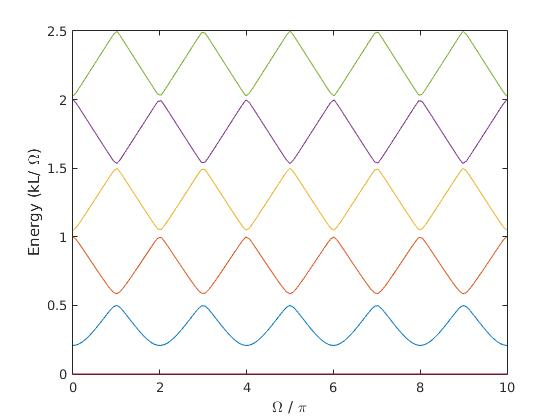
\includegraphics[ scale = 0.3]{cross.jpg}
\end{center}\vspace*{-10pt}\caption{Plot of the energy spectrum for each particle from rotational speed of 0 to $10 \pi$. In this case, $k$ is an integer value related to each respective energy level. With a barrier present, there are avoided crossings at intervals of $\pi$ that increase as a function of barrier strength.}
\label{fig:avoid}
\end{figure}

 In general, quantum optimal control techniques use a given Hamiltonian with a number of control parameters to determine the control parameters' dependence on time. In this case, this means that we will be using the given Hamiltonian to determine the most efficient way to stir our system in order to produce a macroscopic superposition state instead of an oscillation between the two angular momentum states. In particular the Chopped RAndom-Basis quantum optimization (CRAB) optimal control technique has been implemented in this project \cite{CRAB}.


\section*{The CRAB technique}
In order to maximize the fidelity at the avoided crossings, we need to find the optimal (non-adiabatic) rotational pulse as a function of time from 0 to $\pi$, the location of the avoided crossing. With the CRAB optimal control technique, the rotation of our barrier will be:
$$\Gamma^{CRAB}_j(t) = \Gamma^0_j(t)g_j(t)$$
$\Gamma^0_j$ is an initial guess we provide that is modified by $g_j(t)$, the function to be optimized:
$$g(t) = 1 + \frac{\sum^{N}_{n = 0}A_n\sin(\omega_nt)+B_n\cos(\omega_nt)}{\lambda(t)}$$
Where $\lambda(t)$ is a function, chosen such that $\lambda(t) \rightarrow \infty$ for $t \rightarrow 0$ and $t \rightarrow T$. In our implementation, $$\lambda(t) = \frac{T^2}{4t(t-T)}$$  The values of $A$, $B$, and $\omega$ are first randomly assigned, then optimized based on the output infidelity with a minimization algorithm, such as the Nelder--Mead method \cite{SIMPLEX}. 

With the CRAB technique, our  guess-pulse is continually modified by sine and cosine functions of varying intensities and frequencies until all the simplex points converge on a single fidelity value.

\begin{figure*}
\begin{center}
	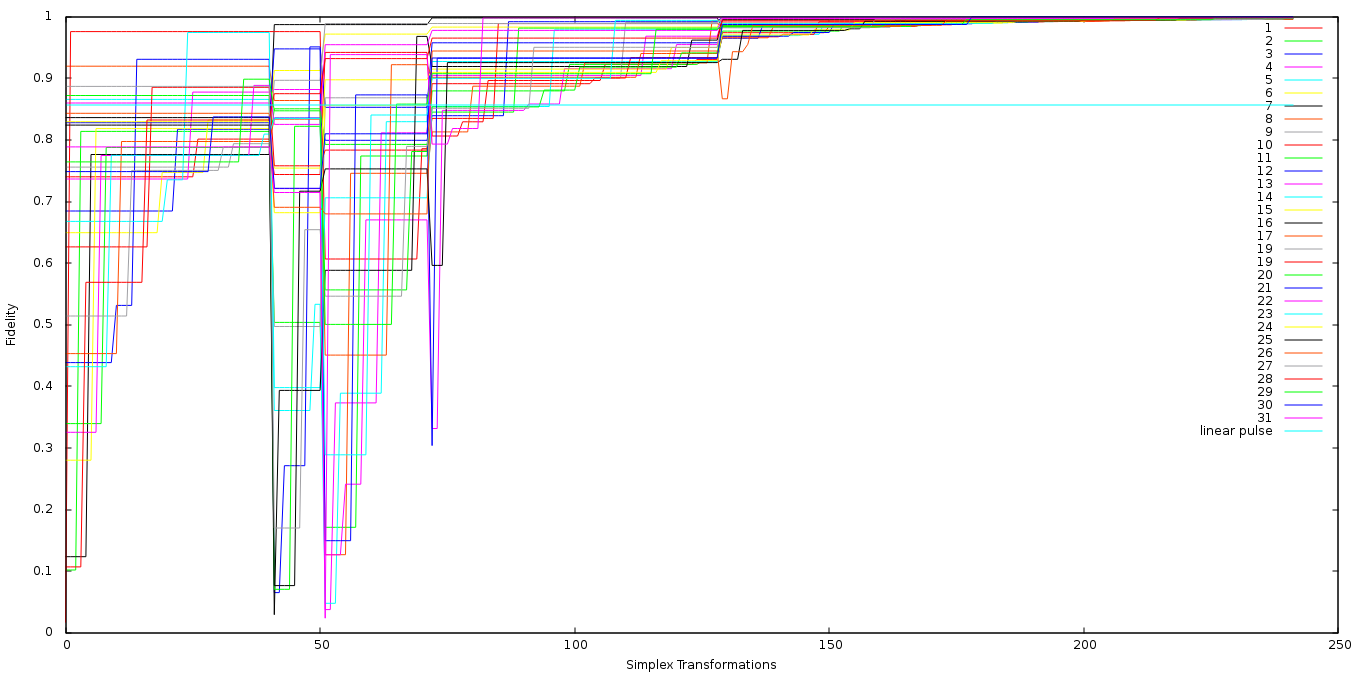
\includegraphics[ scale = 0.25]{fidelities_real.png}
\end{center}\vspace*{-10pt}\caption{Plot of the fidelities of each set of parameters ($N = 10$) as they converge to a value of 0.9995. The total evolution time of this simulation is 20 $\frac{mL^2}{\pi\hbar}$. The $\Omega(t)$ for these fidelities are shown in Figure~\ref{fig:pulse}. The fidelity of a linear pulse is also shown. Note that the fidelity of every simplex point surpasses that of the linear pulse after roughly 100 simplex transformations.}
\label{fig:fid}
\end{figure*}


\section*{Implementation}

A single rotational pulse from our implementation of the CRAB optimal control technique with $N = 10$ and a total simulation time of $20 \frac{mL^2}{\pi\hbar}$ is shown in Figure~\ref{fig:pulse}, and the varying fidelities of each point in this simulation's 31 point simplex before converging are shown in Figure~\ref{fig:fid}. Note that the pulse shape shown in Figure~\ref{fig:pulse} may come as a surprise, as the rotational speed ascends and descends far above a linear pulse to find a desired fidelity close to unity.

Note that in this report, we have used only a single particle on our ring. In all simulations, our original guess pulse is linear from 0 to $\pi$ over some variable simulation time. The longer the simulation time, the closer the pulse is to the adiabatic regime, where the ultracold atoms remain at the ground state at all times. The final fidelity of all of our pulses, then, increases with the simulations time we allow our ring to realize an angular velocity of $\pi$, shown in Figure~\ref{fig:lfid}.

\section*{Closing remarks}

We have implemented the CRAB optimal control technique \cite{CRAB}, using the Nelder--Mead minimization method \cite{SIMPLEX}, for a single particle on a ring with a rotating barrier \cite{RING} to achieve a $\ket{0}+\ket{1}$ state. For this, we determined the optimal angular velocity of the barrier as a function of time, starting at 0 and finishing at $\pi$, the position of the first avoided crossing (Figure~\ref{fig:avoid}). At that point, our implementation of the CRAB algorithm maximizes the fidelity. In the future, it may be worthwhile to study the effects of changing additional parameters, such as the barrier strength, with time or implement multiple particles and study effects of the Tonks-Girardeau gas. It should be now possible to generate a rotating pulse in a certain time regime to create a ``NOON" state on a ring with a rotating barrier.
 

%-------------------------------------------------------------------------------
% RESOURCES
%-------------------------------------------------------------------------------

\section*{Resources}
This code has been written in MATLAB and can be found on the internal git repository of the Cool Stuff Unit. Please contact us if you wish to use the code for any purpose.

\begin{thebibliography}{99} % Bibliography - this is intentionally simple in this template

\bibitem[1]{CRAB} T. Caneva, T. Calarco, S. Montangero,
    \newblock{\em Phys. Rev. A}, 84:022326 (2011).
\vspace*{-10pt}
\bibitem[2]{RING} D. Hallwood, T. Ernst, and J. Brand,
    \newblock {\em Phys. Rev. A}, 82:063623 (2010).
\vspace*{-10pt}
\bibitem[3]{CROSSING} C. Shenke, A. Minguzzi, and F. Hekking,
    \newblock {\em Phys. Rev. A}, 85:053627 (2012).
\vspace*{-10pt}
\bibitem[4]{SIMPLEX} J. Nelder and R. Mead,
    \newblock {\em The Computer Journal}, 7:308. (1965).
\vspace*{-10pt}
\bibitem[5]{OC} P. Doria, T. Calarco, and S. Mantangero,
    \newblock {\em Phys. Rev.}, 106:190501 (2011).
\end{thebibliography}

%-------------------------------------------------------------------------------


\end{document}